%
% teil1.tex -- Beispiel-File für das Paper
%
% (c) 2020 Prof Dr Andreas Müller, Hochschule Rapperswil
%
% !TEX root = ../../buch.tex
% !TEX encoding = UTF-8
%
\section{Lineares Medium\label{particles:section:linear}}
\kopfrechts{Lineares Medium}
% TODO: Quellenangaben
% [ ]: https://en.wikipedia.org/wiki/Linearity
% [ ]: Lineare Algebra: Eine anwendungsorientierte Einführung, Seite: 27, ISBN: 978-3-662-67865-7, Published: 01 September 2023, DOI: https://doi.org/10.1007/978-3-662-67866-4

\subsection{Was ist Linearität?}
Für den einfachsten und üblichsten Fall nimmt man oft ein \emph{lineares Medium} an.
Solch ein Medium nennt man \emph{linear}, wenn dessen Definition sowohl \emph{additiv}
\[
    f(x_{1} + y_{1}, \ldots, x_{n} + y_{n}) 
    = 
    f(x_{1}, \ldots, x_{n}) 
    + 
    f(y_{1}, \ldots, y_{n}),
\]
als auch \emph{homogen}
\[
    f(\lambda x_{1}, \ldots, \lambda x_{n}) 
    = 
    \lambda f(x_{1}, \ldots, x_{n})
\]
ist.

In der Wellentheorie bedeutet dies, 
dass die Materialeigenschaften --- beispielsweise die Elastizität --- nicht von der Amplitude der Welle abhängen.
Diese Elastizität eines Mediums lässt sich durch das \emph{hookesche Gesetz}
\[
    \Delta l
    = 
    \frac{F}{D}
    \label{particles:eq:hookesches-gesetz},
\]
welches bereits in \autoref{chapter:elastomechanik} verwendet wurde, beschreiben.
Dabei beschreibt $\Delta l$ die Veränderung der Distanz zwischen zwei Punkten,
$F$ die dazwischen wirkende Kraft und $D$ einen Proportionalitätsfaktor, 
welcher für den einfachen Fall konstant ist. Also gilt 
\[
    \frac{\partial D}{\partial F} 
    \overset{!}{=} 
    0 
    \quad 
    \forall F.
\]
Mittels Substitution kann man nun darauf schliessen, 
dass es sich hierbei tatsächlich um eine lineare Funktion handeln muss.

\begin{figure}
    \centering
    \subfigure[]{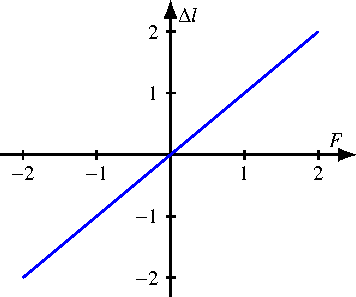
\includegraphics{./papers/particles/figures/out/lineares_medium_deformation.pdf}\label{particles:fig:lin-medium:deform}}\hfill
    \subfigure[]{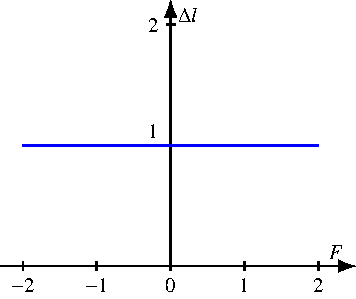
\includegraphics{./papers/particles/figures/out/lineares_medium_elast_modul.pdf}\label{particles:fig:lin-medium:elast-modul}}
    \caption{Deformation~(a) und Elastizitätsmodul~(b) eines linearen Mediums mit konstantem Faktor $D = 1$.}
\end{figure}

\subsection{Superpositionsprinzip}\label{particles:section:lin-medium:superposition} % TODO: Subsection umschreiben
Das Superpositionsprinzip fasst die Bedingungen zur Linearität nochmal etwas schöner in eine Formel zusammen, 
nämlich
\[
    T(\lambda x + \mu y)
    = 
    \lambda T(x) 
    + 
    \mu T(y).
\]
Blickt man wieder auf die Wellentheorie, so bedeutet dies, 
dass sich Wellen in linearen Medien überlagern, 
sich aber nicht gegenseitig beeinflussen.
Dies kann man schön anhand zweier sich kreuzende Strahlen im Vakuum veranschaulichen, 
wie sie in \autoref{particles:fig:lin-medium:beams} gezeigt werden.
Lokal interferieren diese Strahlen zwar, stören jedoch nicht wirklich ihren weiteren Verlauf.
\begin{figure}
    \centering
    \subfigure[]{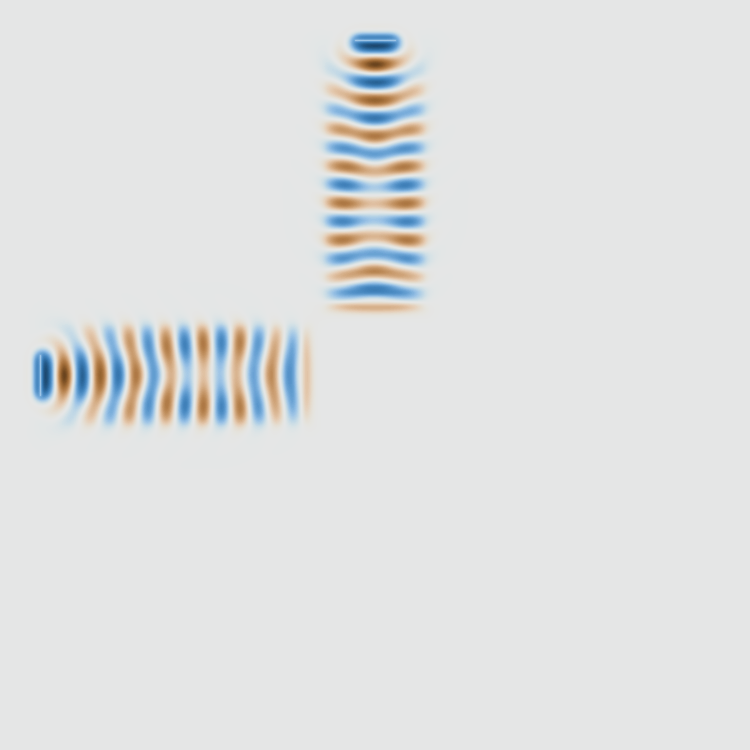
\includegraphics[width=.32\linewidth]{./papers/particles/figures/simulations/beams_lin_1_10.png}}\label{particles:fig:lin-medium:beams-1}\hfill
    \subfigure[]{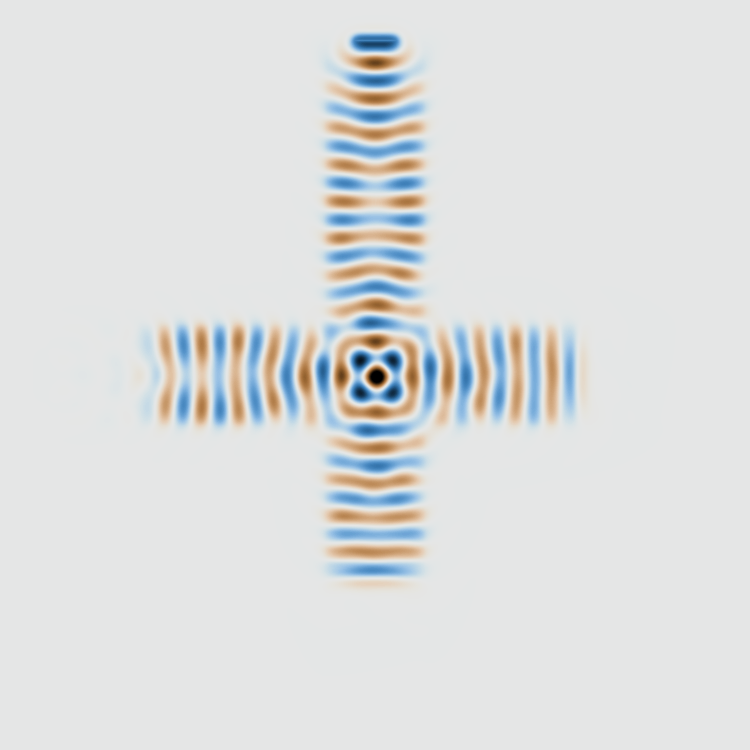
\includegraphics[width=.32\linewidth]{./papers/particles/figures/simulations/beams_lin_3_20.png}}\label{particles:fig:lin-medium:beams-2}\hfill
    \subfigure[]{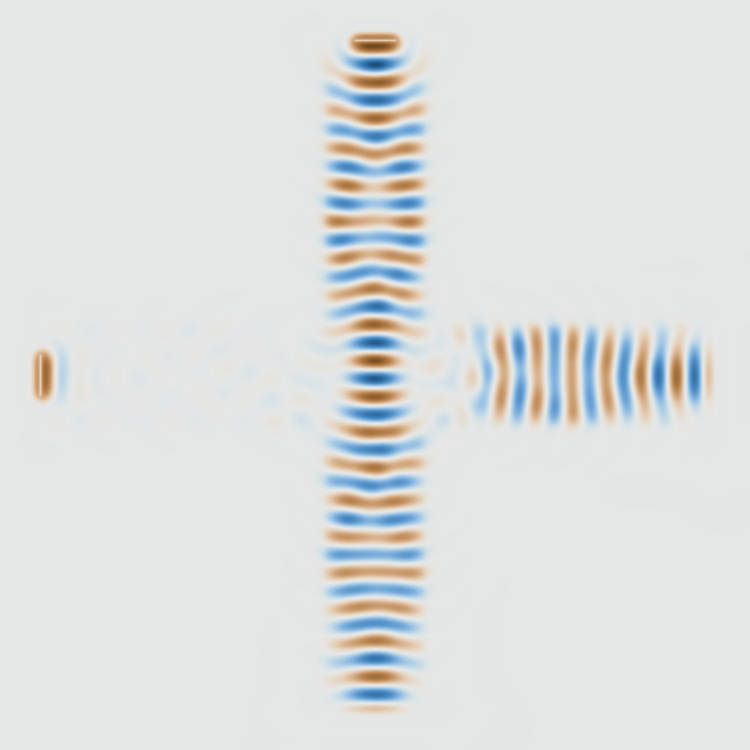
\includegraphics[width=.32\linewidth]{./papers/particles/figures/simulations/beams_lin_4_32.png}}\label{particles:fig:lin-medium:beams-3}
    \caption{Strahlen im linearen Medium zu Beginn~(a), während sie sich kreuzen~(b), und danach~(c).}\label{particles:fig:lin-medium:beams}
\end{figure}


\subsection{Wellengleichung}\label{particles:section:lin-medium:wellengleichung}
Die Wellengleichung 
\begin{equation}
    \frac{\d^2 u}{\d t^2} = c^2 \cdot \nabla^2 u, \label{particles:eq:wellengleichung}
\end{equation}
hat in vielen Feldern Anwendung.
Dabei steht auf der linken Seite die zweite Ableitung nach der Zeit und auf der rechten die räumliche Ableitung sowie die Konstante $c^2$.
Eine massgebende Annahme ist dabei die Linearität des Mediums.
Dies wird ersichtlicher, wenn man die Herleitung der Wellengleichung beispielsweise aus den Maxwell-Gleichungen betrachtet.
Die dafür verwendeten Maxwell-Gelichungen wurden im Abschnitt~\ref{maxwell:section:teil0} bereits vorgestellt.


\subsubsection{Herleitung}
Zur Herleitung der Wellengleichung im elektrischen Feld ist die Identität
\begin{equation}
    \nabla \times \nabla \times \boldsymbol{U} = \nabla(\nabla \cdot \boldsymbol{U}) - \nabla^2 \boldsymbol{U}\label{particles:eq:rot-identity}
\end{equation}
notwendig. 
Diese wurde in Abschnitt~\ref{buch:vektoranalysis:subsection:rotrot} als Gleichung~\eqref{buch:vektoranalysis:eqn:rotrot} bereits hergeleitet und gilt für beliebige Vektorfelder.

Als erster Schritt der Herleitung wird $\rho = 0$, also ein Medium ohne freie Ladungsträger, angenommen.
Das gausssche Gesetz
\[
    \nabla \cdot \boldsymbol{D} = \rho_\text{frei},
\]
wie es in Gleichung~\eqref{maxwell:equation:gauss} gezeigt wurde, wird unter dieser Annahme zu
\begin{equation}
    \nabla \cdot \boldsymbol{D} = 0.\label{particles:eq:gauss}
\end{equation}
Weiter wird der erweiterte Durchflutungssatz
\[
    \nabla \times \boldsymbol{H} = \boldsymbol{j}_\text{frei} + \frac{\d \boldsymbol{D}}{dt}
\]
aus Gleichung~\eqref{maxwell:equation:durchflutungssatz} durch Annahme einer Stromdichte von $\boldsymbol{j}_\text{frei} = 0$ zu
\begin{equation}
    \nabla \times \boldsymbol{H} = \frac{\d \boldsymbol{D}}{dt}.\label{particles:eq:durchflutungssatz}
\end{equation}
Es ist anzumerken, dass in Gleichung~\eqref{maxwell:equation:durchflutungssatz} bereits die weiter unten in den Gleichungen~\ref{particles:eq:de} und~\ref{particles:eq:bh} gezeigten Verhältnisse eingesetzt wurden.
Das Induktionsgesetz
\begin{equation}
    \nabla \times \boldsymbol{E} = -\frac{\d \boldsymbol{B}}{\d t}\label{particles:eq:induktionsgesetz},
\end{equation}
das als Gleichung~\eqref{maxwell:equation:induktionsgesetz} vorgestellt wurde, wird ebenfalls benötigt.

Um die elektrische Flussdichte $\boldsymbol{D}$ mit dem elektrischen Feld $\boldsymbol{E}$ in Relation zu bringen, 
wird die Permittivität $\varepsilon$ beigezogen.
Die Permittivität ist abhängig vom Medium. 
$\boldsymbol{D}$ und $\boldsymbol{E}$ stehen also im Verhältnis
\begin{equation}
    \boldsymbol{D} = \varepsilon \boldsymbol{E}.
    \label{particles:eq:de}
\end{equation}
Ein ähnliches Verhältnis stellt sich zwischen der magnetischen Flussdichte $\boldsymbol{B}$ und der magnetischen Feldstärke $\boldsymbol{H}$ ein, wobei das Verhältnis durch die Permeabilität $\mu$ als
\begin{equation}
    \boldsymbol{B} = \mu \boldsymbol{H} \quad \text{bzw.} \quad \boldsymbol{H} = \frac{\boldsymbol{B}}{\mu}
    \label{particles:eq:bh}
\end{equation}
gegeben wird.
Auch die Permeabilität ist abhängig vom Medium.

Zunächst wird das Induktionsgesetz~\eqref{particles:eq:induktionsgesetz} durch die Rotation zu
\begin{align}
    \nabla \times \nabla \times \boldsymbol{E} 
        &= - \nabla \times \frac{\d\boldsymbol{B}}{\d t} \\
        &= - \frac{\d}{\d t} \nabla \times \boldsymbol{B}
\end{align}
erweitert.
Mit der Identität~\eqref{particles:eq:rot-identity} und der Permeabilität kann das Resultat zu
\[
    \nabla(\nabla \cdot \boldsymbol{E}) - \nabla^2 \boldsymbol{E} = -\mu \frac{\d}{\d t} \nabla \times \boldsymbol{H}
\]
umgeformt werden.
Durch Einsetzen des gaussschen Gesetzes~\eqref{particles:eq:gauss} und dem Durchflutungssatz~\eqref{particles:eq:durchflutungssatz} entsteht
\[
    - \nabla^2 \boldsymbol{E} = -\mu \frac{\d}{\d t} \frac{\d \boldsymbol{D}}{\d t}
\]
und schliesslich entsteht mit $\boldsymbol{D} = \varepsilon \boldsymbol{E}$
\[
    \nabla^2 \boldsymbol{E} = \mu\varepsilon \frac{\d^2 \boldsymbol{E}}{\d t^2} 
    \quad \text{bzw.} \quad
    \frac{\d^2 \boldsymbol{E}}{\d t^2} = \frac{1}{\mu \varepsilon} \nabla^2 \boldsymbol{E},
\]
was der Wellengleichung entspricht.
Durch ähnliches Vorgehen kann diese auch für die magnetische Feldstärke $\boldsymbol{B}$ hergeleitet werden.

Durch Parametervergleich mit der Wellengleichung aus~\eqref{particles:eq:wellengleichung} wird klar, dass die Ausbreitungsgeschwindigkeit
\[
    c = \frac{1}{\sqrt{\mu\varepsilon}}\label{particles:eq:lichtgeschwindigkeit}
\]
beträgt.
Damit die Gleichung gut analytisch lösbar ist, sollten die beiden Faktoren $\mu$ und $\varepsilon$ also über verschiedene Feldstärken konstant sein.
Ansonsten wird aus der linearen partiellen Differenzialgleichung eine nichtlineare.


\subsection{Schwinger-Limit}\label{particles:section:lin-medium:schwinger}
Es wird erwartet, dass bei extrem hohen Feldstärken selbst das Vakuum nichtlinear wird.
Dieser Übergang zur Nichtlinearität des Vakuums wurde erstmals im Jahre 1951 von Fritz Sauter in der \emph{Zeitschrift für Physik}~\cite{particles:fritz_sauter} theoretisiert.
Julian Schwinger arbeitete diese Idee im Paper \emph{On Gauge Invariance and Vacuum Polarization}~\cite{particles:schwinger-limit} weiter aus, 
weshalb die Grenze schliesslich nach ihm benannt wurde.
Da es sich hierbei um elektrische und magnetische Feldstärken im Bereich von $10^{18}\,\frac{\text{V}}{\text{m}}$ und $10^9\,\text{T}$ handelt, 
konnte dieses Limit bisher noch nicht gemessen werden.
Entsprechend ist das Schwinger-Limit noch immer Bestandteil aktueller Forschungen, 
wie das Paper \emph{Observing Light-by-Light Scattering at the Large Hadron Collider}~\cite{particles:photon_photon_scattering} zeigt.
Es wird darin die Photonen-Photonen-Streuung beobachtet, was ein starkes Indiz dafür ist, 
dass das Schwinger-Limit tatsächlich existiert.
Zudem taucht das Limit bei weiteren Experimenten wie zum Beispiel dem ATLAS-Experiment~\cite{particles:atlas-experiment}, 
welche sich mit extrem starken Feldstärken befassen, öfters als Nebenprodukt auf.

Beschränkt man sich jedoch nicht nur auf das Vakuum, so findet man Medien, 
welche bereits bei deutlich kleineren Feldstärken nichtlineare Eigenschaften aufweisen.
Ein Beispiel von solchen nichtlinearen Werkstoffen sind, 
wie~\cite{particles:frequenzverdopplung} demonstriert, Kristalle zur Frequenzverdoppelung.
Diese werden beispielsweise in grünen Laserpointern eingesetzt, 
was die Verwendung von preiswerteren Infrarot-Laserdioden anstelle der teureren grünen Ausführung erlaubt.
